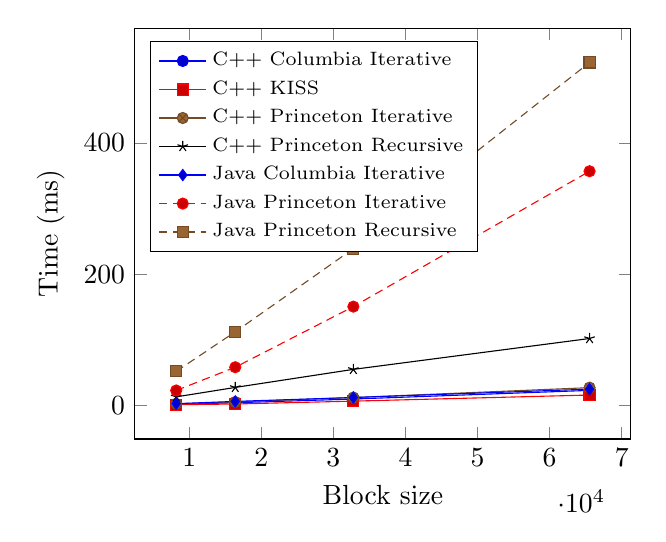
\begin{tikzpicture}
\begin{axis}[xlabel={Block size},ylabel={Time (ms)},width=0.65\linewidth,legend pos=north west,scaled y ticks = false,legend cell align=left,legend style={font=\scriptsize}]
\addplot coordinates {
(8192, 1.9326)
(16384, 4.2789)
(32768, 9.9388)
(65536, 23.1031)
};
\addplot coordinates {
(8192, 1.2470)
(16384, 2.3713)
(32768, 6.7420)
(65536, 16.0281)
};
\addplot coordinates {
(8192, 2.5845)
(16384, 5.4518)
(32768, 12.2266)
(65536, 27.2805)
};
\addplot coordinates {
(8192, 13.2345)
(16384, 27.6080)
(32768, 55.1227)
(65536, 102.1585)
};
\addplot coordinates {
(8192, 2.8726)
(16384, 6.3214)
(32768, 12.2634)
(65536, 24.9874)
};
\addplot coordinates {
(8192, 22.9609)
(16384, 58.3825)
(32768, 150.7299)
(65536, 356.9871)
};
\addplot coordinates {
(8192, 52.0853)
(16384, 112.3024)
(32768, 239.0777)
(65536, 522.7409)
};
\legend{C++ Columbia Iterative,C++ KISS,C++ Princeton Iterative,C++ Princeton Recursive,Java Columbia Iterative,Java Princeton Iterative,Java Princeton Recursive}
\end{axis}
\end{tikzpicture}
